\emph{(This is the follow-up to the first article, published October
9th, On Advertising: Part 1 - Before~which explores the hows and whys of
our little experiment in advertising. ~Start there if you have yet to
read it!)}

And so it's over. ~We ran advertisements for one month on two furry
sites to try and gain some insight into the way furries interact both
with ads and with those sites in general. Those campaigns ended several
days ago and we've been looking over the data we have available to us,
including information before, during, and after the campaigns were over.

Let's take a look, shall we?

\subsection{{[}adjective{]}{[}species{]}}\label{adjectivespecies}

\begin{figure}[htbp]
\centering
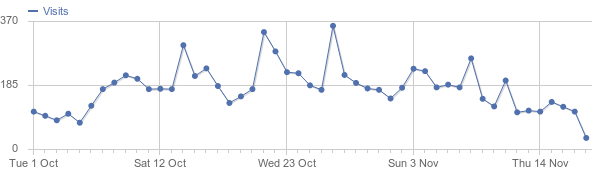
\includegraphics{/assets/furry/ads/as-postads.png}
\caption{{[}adjective{]}{[}species{]} post-ads}
\end{figure}

Campaign

Visits

furaffinity

1486

sofurry

174

As with any site with a publishing schedule such as ours, one can expect
the spikes around the days when articles go live. ~That was true before,
as well as during and after the advertising campaign. ~In fact, though
there is a visible increase in the average number of visitors, and the
campaigns do show some activity*, this ad was less effective than both
the Love - Sex - Fur and Furry Poll ads. ~I think that this was due to
the relatively calm and passive nature of the advertisement itself.
~While LSF's ad was also passive in nature, it did happen to include the
word `sex' as well as a salacious RandomWolf in red-tinted glasses
(ain't he dreamy?). ~The Furry Poll ad, on the other hand, was more of a
call to action, using very active language such as ``Take part\ldots{}''
and ``Stand up - Get counted!''.

However, these numbers aren't the only ones worth taking a look at. ~In
addition to the increase in visitors, the {[}adjective{]}{[}species{]}
FurAffinity account has gained 81 new watchers (and one spam note
offering free anime downloads!), and the Twitter account at least 40 new
followers (Twitter will only let me look back so far). ~Even more
surprising, to me, was that my own personal FA account gained 30 new
followers. ~JM reports that he has also seen an increase in followers on
FA. ~The amount of times that we have been contacted via shouts,
notes**, and emails has increased, as well. ~Several of those who have
found us (or perhaps even already knew about us) have some delightful
ideas worth exploring within the fandom, it seems!

\subsection{Love - Sex - Fur}\label{love---sex---fur}

\begin{figure}[htbp]
\centering
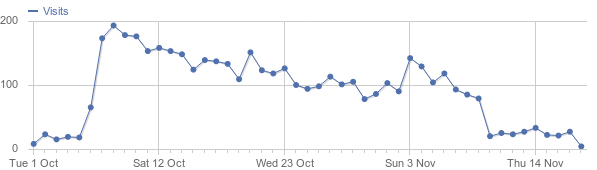
\includegraphics{/assets/furry/ads/lsf-postads.png}
\caption{Love - Sex - Fur post-ads}
\end{figure}

Campaign

Visits

furaffinity

3440

sofurry

258

\href{http://lovesexfur.com}{LSF}'s activity is, of course much lower
than {[}a{]}{[}s{]}'s. ~I have been on something of a sabbatical*** (as
I did around this time last year), and JM has been extraordinarily
helpful in carrying the burden of {[}adjective{]}{[}species{]}, but
there hasn't been as much traffic to Love - Sex - Fur, understandably.
Along with 42 new watchers on FA, 24 new Twitter followers, and another
note received there, we can more easily see the effect of advertising on
site traffic without the spikes of new articles being posted on a
regular basis.

\subsection{The Furry Poll}\label{the-furry-poll}

\begin{figure}[htbp]
\centering
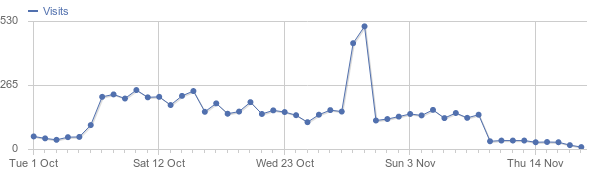
\includegraphics{/assets/furry/ads/furrypoll-postads.png}
\caption{The Furry Poll post-ads}
\end{figure}

Campaign

Visits

furaffinity

3440

sofurry

258

Whoa there! ~Although this graph shows pretty clearly the start and end
of the ad campaign, the numbers are skewed by the graph's scaling due to
a very large jump on October 29th and 30th. ~As far as is visible from
the referrers list during that time, the survey was shared in two large
furry groups on Facebook (which ones are, of course, not visible to us).

The presence of furries on Facebook has always felt somewhat surprising
to me. ~I do not shrink from sharing my membership with this subculture
in contexts outside of the fandom. ~I go by Makyo on work's IRC servers,
I use the same old dapper-fox-drinking-a-gin-and-tonic icon on GitHub,
where some of our code is stored, and I've even used one of the
{[}a{]}{[}s{]} visualizations to prove a point about overwhelming
amounts of data during a meeting. ~Something about the way that Facebook
promotes unmediated sharing and monetizing of information rubs me the
wrong way, however. ~Perhaps this is a holdover from my early-adopter
days, when Facebook was touted as the best way for students to connect
and share photos and such with each other, when it was restricted to
university students. ~For me, the site still feels like the very mundane
(in all senses of the term) social media network, focused primarily on
staying in touch with classmates.

However, I know that's not the case, as I've seen several incoming
spikes such as this show up from links being shared on Facebook. ~For
those of you who are active in a furry context on Facebook, how do you
manage your identity there? ~Do you have a separate furry-only profile,
or do you mix in all circles with one profile?

And to whomever shared a link to the furry survey on Facebook, cheers!
~Of all of the sites included in this exercise, the survey is the one
that will benefit the most from increased exposure. It's important that
we get as many responses from all around the world as possible to
provide a clearer picture of our community. ~Given the single-use nature
of the survey site, the dramatic decrease in numbers after the
campaign's end is not too surprising: after all, there's no reason to
revisit the site more than once a year!

\subsection{Bookmarfs!}\label{bookmarfs}

\begin{figure}[htbp]
\centering
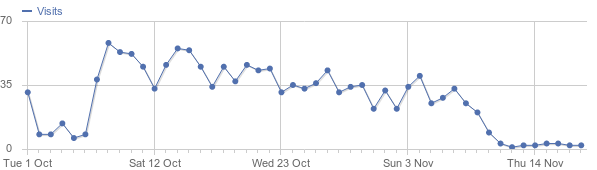
\includegraphics{/assets/furry/ads/bookmarfs-postads.png}
\caption{Bookmarfs! post-ads}
\end{figure}

Campaign

Visits

furaffinity

1017

sofurry

117

\href{http://bookmarfs.com}{Bookmarfs!} is an unrelated project, but one
that also needed an advertisement. Additionally, once I noticed that all
of our ads followed the same format, I took a different path with this
one: no striped background, simple and to the point. ~The ad was
actually strikingly effective during the period it was shown, given the
relatively low initial interest and the (current) rate at which we post:
twice a month, usually on the same day - once for the discussion of the
past month's book and once to announce the next month's book. ~We also
received 14 new watchers on FA and 10 new followers on Twitter.

\subsection{Conclusions}\label{conclusions}

I think that the advertising experiment was useful in seeing just how
the fandom utilizes advertising. ~Judging by personal interactions with
friends and through comments here on the previous post, our reaction to
advertising is decidedly mixed. ~Several people I have heard from have
described ads in general to be intrusive and a nuisance, especially on
the Internet. ~However, I am not the only one who turns off ad-blockers
on furry sites such as FurAffinity and SoFurry. ~Part of it is that I
know that a higher percentage of ads are, by the very virtue of their
existence on these sites, targeted toward my interests. ~However, and
I'm not alone in thinking this way, it's also good to know that a lot of
the people posting these ads are individuals, sharing an interest in
common with me, who are doing their best to get by in life doing
something they love.

This, in fact, is one of the reasons that I ran these ads only in
month-long intervals. ~{[}adjective{]}{[}species{]} projects (and
Bookmarfs!) are all projects run out of pocket with no profit incentive.
~We sell no products or services, and we write because that's what we
love to do. ~Our readership is fantastic, and we would love to grow
that, but it's also nice to give the space to the creators who are doing
their best to make a living in our little subculture.

Advertising~does play a role in our community, and I think that these
few examples have shown just how that information is transmuted into a
measurable and visible change. ~For those out there questioning whether
or not their business within furry will benefit from advertising, I
think this serves as a fairly strong ``yes''. ~I placed four ads on two
high-traffic sites for a month for just about \$130 (about the cost of
running all of the above sites except for the furry survey for one year)
and the results were immediate.

\begin{center}\rule{0.5\linewidth}{\linethickness}\end{center}

* The campaign numbers differ significantly from the impressions
reported by SoFurry's advert system (campaign reports 174 impressions,
SoFurry reports 429 clicks for {[}a{]}{[}s{]}, with similar skews for
other sites). ~Piwik, our metrics tool, plays nice with AdBlock,
Noscript, and other such tools, and so there are likely several more
visitors than are actually being reported by these metrics. ~However, it
was still nice to get an idea of the ways in which advertising works
within our community!

Here are the actual numbers from SoFurry:

\begin{figure}[htbp]
\centering
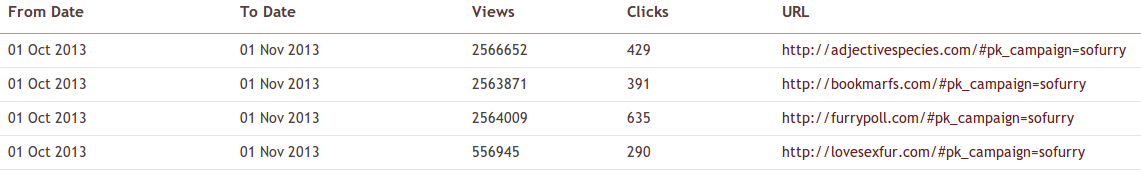
\includegraphics{/assets/furry/ads/sofurry-results.png}
\caption{SoFurry results}
\end{figure}

** In general, notes are a poor way to get in touch with us. ~Please
email instead!

*** Apologies for the paucity of content on my part! ~However, I will be
attending Mid-West Fur Fest this year, so if you catch me around, I'd be
more than happy to talk shop, furry or otherwise!
